\documentclass[aspectratio=169,10pt,fontset=fandol]{ctexbeamer}
\usepackage{amsmath,amssymb,mathtools,bm,mathrsfs}
\usepackage{graphicx,booktabs,array,tabularx,multirow}
\usepackage{tikz,pgfplots,xparse,xstring,mdframed}
\usetikzlibrary{arrows.meta,calc,angles,positioning,shapes.geometric,graphs}
\pgfplotsset{compat=1.18}
\usetheme{fduclassroom}
\input{workflow_style.tex}
\input{workflow_fonts.tex}
\newenvironment{proofdetail}{\par\noindent\textbf{证明：}\quad}{\par}
\renewenvironment{solution}{\par\noindent\textbf{解：}\quad}{\par}
\mdfdefinestyle{extrastyle}{%
    linecolor=gray,
    linewidth=0.8pt,
    frametitlerule=true,
    frametitlebackgroundcolor=gray!10,
    backgroundcolor=gray!5,
    skipabove=10pt,
    skipbelow=10pt,
    innertopmargin=6pt,
    innerbottommargin=6pt
}
\newenvironment{extra}{\begin{mdframed}[style=extrastyle, frametitle={* 选读内容（不要求掌握）}]}{\end{mdframed}}
\newenvironment{custom}[1]{\par\noindent\textbf{#1}\quad}{\par\vspace{0.8em}}
\newenvironment{idea}{\par\noindent\textbf{思路}\quad}{\par\vspace{0.4em}}
\newenvironment{warning}{\par\noindent\textbf{注：}\quad}{\par\vspace{0.8em}}
\newenvironment{intuition}{\par\noindent\textbf{直观理解}\quad}{\par\vspace{0.8em}}
\NewDocumentEnvironment{application}{O{}}
{\par\noindent\textbf{应用拓展\IfStrEq{#1}{}{}{——#1}}\quad}
{\par\vspace{0.8em}}
\newcommand{\dd}{\mathrm{d}}
\newcommand{\ee}{\mathrm{e}}
\newcommand{\ii}{\mathrm{i}}
\newcommand{\RR}{\mathbb{R}}
\newcommand{\upcite}[1]{\textsuperscript{\textsuperscript{\cite{#1}}}}
\DeclareMathOperator*{\argmax}{\mathrm{arg\,max}}
\DeclareMathOperator*{\argmin}{\mathrm{arg\,min}}
\title{第三章完整应用流程验收}
\begin{document}
\section{一元函数极限}
% FRAME-ID F001
\begin{frame}[t,fragile]{目录}
\normalsize
{\color{blue}\normalsize 1. 一元函数极限\par}\vspace{0.22em}
{\color{gray!40}\normalsize 2. 函数极限的基本性质\par}\vspace{0.22em}
{\color{gray!40}\normalsize 3. 两个重要极限\par}\vspace{0.22em}
{\color{gray!40}\normalsize 4. 等价无穷小\par}\vspace{0.22em}
{\color{gray!40}\normalsize 5. 一元函数的连续性\par}\vspace{0.22em}
{\color{gray!40}\normalsize 6. 闭区间连续函数的两个基本定理\par}\vspace{0.22em}
{\color{gray!40}\normalsize 7. 二元函数的极限与连续\par}\vspace{0.22em}
\end{frame}
% FRAME-ID F002
\begin{frame}[t,fragile]{一元函数极限}
\normalsize
{\normalsize
% SOURCE-BEGIN U0002 0 166
数列极限研究的是离散点列 \(a_1,a_2,\ldots\) 的变化趋势；函数极限研究的则是自变量在某个点附近连续变化时，函数值的变化趋势。讨论 \(x\to x_0\) 时，只关心 \(x\) 充分接近 \(x_0\) 且 \(x\neq x_0\) 的情形，这一区域称为 \(x_0\) 的\textbf{去心邻域}。


% SOURCE-END U0002
}
\end{frame}
% FRAME-ID F003
\begin{frame}[t,fragile]{一元函数极限}
\normalsize
\begin{block}{定义}
{\normalsize
% SOURCE-BEGIN U0003 0 277
\textbf{函数极限的\(\varepsilon\)--\(\delta\) 语言}\par

设函数 \(f\) 在点 \(x_0\) 的某个去心邻域内有定义。若存在常数 \(A\)，使得对任意 \(\varepsilon>0\)，总存在 \(\delta>0\)，当
\[
0<|x-x_0|<\delta
\]
时都有
\[
|f(x)-A|<\varepsilon,
\]
则称当 \(x\to x_0\) 时 \(f(x)\) 的极限为 \(A\)，记作
\[
\lim_{x\to x_0}f(x)=A.
\]

% SOURCE-END U0003
}
\end{block}
\end{frame}
% FRAME-ID F004
\begin{frame}[t,fragile]{一元函数极限}
\normalsize
{\normalsize
% SOURCE-BEGIN U0004 0 112
定义中的逻辑次序是“先给误差要求 \(\varepsilon\)，再寻找自变量范围 \(\delta\)”。\(\delta\) 可以依赖于 \(\varepsilon\)，但不能依赖于邻域中临时选取的 \(x\)。


% SOURCE-END U0004
}
\end{frame}
% FRAME-ID F005
\begin{frame}[t,fragile]{一元函数极限}
\normalsize
\begin{block}{例题}
{\normalsize
% SOURCE-BEGIN U0005 0 60
\textbf{按定义证明函数极限}\par

证明
\[
\lim_{x\to2}(3x-1)=5.
\]

% SOURCE-END U0005
}
\end{block}
\end{frame}
% FRAME-ID F006
\begin{frame}[t,fragile]{一元函数极限}
\normalsize
{\normalsize
\textbf{证明：}
% SOURCE-BEGIN U0006 0 178
任取 \(\varepsilon>0\)。注意到
\[
|(3x-1)-5|=3|x-2|.
\]
取 \(\delta=\varepsilon/3\)，则当 \(0<|x-2|<\delta\) 时，
\[
|(3x-1)-5|<3\delta=\varepsilon.
\]
因此 \(\lim_{x\to2}(3x-1)=5\)。

% SOURCE-END U0006
}
\end{frame}
% FRAME-ID F007
\begin{frame}[t,fragile]{一元函数极限}
\small
{\small
% SOURCE-BEGIN U0007 0 242
\begin{custom}{极限与函数在该点的取值无关}
函数极限只考察去心邻域，所以 \(f(x_0)\) 可以等于极限、不同于极限，甚至没有定义。例如
\[
f(x)=
\begin{cases}
\dfrac{x^2-1}{x-1},&x\neq1,\\
100,&x=1
\end{cases}
\]
满足 \(\lim_{x\to1}f(x)=2\)，尽管 \(f(1)=100\)。改变单独一个点的函数值不会改变该点的极限。
\end{custom}
% SOURCE-END U0007
}
\end{frame}
% FRAME-ID F008
\begin{frame}[t,fragile]{一元函数极限}
\normalsize
{\normalsize
% SOURCE-BEGIN U0008 0 30
\subsubsection*{单侧极限与双侧极限}


% SOURCE-END U0008
}
\end{frame}
% FRAME-ID F009
\begin{frame}[t,fragile]{一元函数极限}
\normalsize
\begin{block}{定义}
{\normalsize
% SOURCE-BEGIN U0009 0 284
\textbf{左极限与右极限}\par

若对任意 \(\varepsilon>0\)，存在 \(\delta>0\)，使得当 \(x_0-\delta<x<x_0\) 时，
\[
|f(x)-A|<\varepsilon,
\]
则称 \(A\) 为 \(f(x)\) 在 \(x_0\) 处的左极限，记作
\[
\lim_{x\to x_0^-}f(x)=A.
\]
类似地，当 \(x_0<x<x_0+\delta\) 时满足上述不等式，则称 \(A\) 为右极限，记作
\[
\lim_{x\to x_0^+}f(x)=A.
\]

% SOURCE-END U0009
}
\end{block}
\end{frame}
% FRAME-ID F010
\begin{frame}[t,fragile]{一元函数极限}
\normalsize
\begin{block}{定理}
{\normalsize
% SOURCE-BEGIN U0010 0 120
\textbf{双侧极限存在的充要条件}\par

\[
\lim_{x\to x_0}f(x)=A
\]
当且仅当
\[
\lim_{x\to x_0^-}f(x)=\lim_{x\to x_0^+}f(x)=A.
\]

% SOURCE-END U0010
}
\end{block}
\end{frame}
% FRAME-ID F011
\begin{frame}[t,fragile]{一元函数极限}
\normalsize
\begin{block}{例题}
{\normalsize
% SOURCE-BEGIN U0011 0 195
\textbf{左右极限不相等}\par

设
\[
f(x)=
\begin{cases}
-1,&x<0,\\
1,&x\geq0.
\end{cases}
\]
则
\[
\lim_{x\to0^-}f(x)=-1,\qquad
\lim_{x\to0^+}f(x)=1.
\]
左右极限不相等，所以 \(\lim_{x\to0}f(x)\) 不存在。

% SOURCE-END U0011
}
\end{block}
\end{frame}
% FRAME-ID F012
\begin{frame}[t,fragile]{一元函数极限}
\normalsize
{\normalsize
% SOURCE-BEGIN U0012 0 33
\subsubsection*{自变量趋于无穷与无穷极限}


% SOURCE-END U0012
}
\end{frame}
% FRAME-ID F013
\begin{frame}[t,fragile]{一元函数极限}
\normalsize
\begin{block}{定义}
{\normalsize
% SOURCE-BEGIN U0013 0 197
\textbf{自变量趋于无穷时的有限极限}\par

若对任意 \(\varepsilon>0\)，存在 \(X>0\)，使得当 \(x>X\) 时都有
\[
|f(x)-A|<\varepsilon,
\]
则称 \(\lim_{x\to+\infty}f(x)=A\)。将条件改为 \(x<-X\)，便得到 \(\lim_{x\to-\infty}f(x)=A\) 的定义。

% SOURCE-END U0013
}
\end{block}
\end{frame}
% FRAME-ID F014
\begin{frame}[t,fragile]{一元函数极限}
\normalsize
\begin{block}{例题}
{\normalsize
% SOURCE-BEGIN U0014 0 196
\[
\lim_{x\to+\infty}\frac{2x+1}{x+3}=2.
\]
事实上，
\[
\left|\frac{2x+1}{x+3}-2\right|=\frac5{x+3}.
\]
给定 \(\varepsilon>0\)，取 \(X>\max\{0,5/\varepsilon-3\}\)，当 \(x>X\) 时上式小于 \(\varepsilon\)。

% SOURCE-END U0014
}
\end{block}
\end{frame}
% FRAME-ID F015
\begin{frame}[t,fragile]{一元函数极限}
\normalsize
\begin{block}{定义}
{\normalsize
% SOURCE-BEGIN U0015 0 342
\textbf{无穷极限}\par

若对任意 \(M>0\)，存在 \(\delta>0\)，使得当 \(0<|x-x_0|<\delta\) 时都有
\[
f(x)>M,
\]
则称 \(\lim_{x\to x_0}f(x)=+\infty\)。将 \(f(x)>M\) 改为 \(f(x)<-M\)，便得到极限为 \(-\infty\) 的定义。

将 \(0<|x-x_0|<\delta\) 分别改为 \(x_0-\delta<x<x_0\) 或 \(x_0<x<x_0+\delta\)，就得到相应的单侧无穷极限；将它改为 \(x>X\) 或 \(x<-X\)，就得到 \(x\to+\infty\) 或 \(x\to-\infty\) 时的无穷极限。

% SOURCE-END U0015
}
\end{block}
\end{frame}
% FRAME-ID F016
\begin{frame}[t,fragile]{一元函数极限}
\normalsize
{\normalsize
% SOURCE-BEGIN U0016 0 156
\begin{warning}
“在 \(x_0\) 附近无界”不等于“极限为无穷”。例如 \(f(x)=\frac{\sin(1/x)}{x}\) 在 \(x=0\) 的任意去心邻域内都无界，但函数值正负振荡，既不趋于 \(+\infty\)，也不趋于 \(-\infty\)。
\end{warning}
% SOURCE-END U0016
}
\end{frame}
\section{函数极限的基本性质}
% FRAME-ID F017
\begin{frame}[t,fragile]{目录}
\normalsize
{\color{black}\normalsize 1. 一元函数极限\par}\vspace{0.22em}
{\color{blue}\normalsize 2. 函数极限的基本性质\par}\vspace{0.22em}
{\color{gray!40}\normalsize 3. 两个重要极限\par}\vspace{0.22em}
{\color{gray!40}\normalsize 4. 等价无穷小\par}\vspace{0.22em}
{\color{gray!40}\normalsize 5. 一元函数的连续性\par}\vspace{0.22em}
{\color{gray!40}\normalsize 6. 闭区间连续函数的两个基本定理\par}\vspace{0.22em}
{\color{gray!40}\normalsize 7. 二元函数的极限与连续\par}\vspace{0.22em}
\end{frame}
% FRAME-ID F018
\begin{frame}[t,fragile]{函数极限的基本性质}
\small
\begin{block}{定理}
{\small
% SOURCE-BEGIN U0017 0 61
\textbf{极限的唯一性}\par

若 \(\lim_{x\to x_0}f(x)\) 存在，则其极限值唯一。

% SOURCE-END U0017
}
\end{block}
\pause
{\small
\textbf{证明：}
% SOURCE-BEGIN U0018 0 281
假设 \(f(x)\) 同时以 \(A\) 和 \(B\) 为极限，且 \(A\neq B\)。取
\[
\varepsilon=\frac{|A-B|}{3}.
\]
当 \(x\) 充分接近 \(x_0\) 且 \(x\neq x_0\) 时，同时有
\[
|f(x)-A|<\varepsilon,\qquad |f(x)-B|<\varepsilon.
\]
由三角不等式，
\[
|A-B|\leq |A-f(x)|+|f(x)-B|<2\varepsilon=\frac23|A-B|,
\]
矛盾。因此 \(A=B\)。

% SOURCE-END U0018
}
\end{frame}
% FRAME-ID F019
\begin{frame}[t,fragile]{函数极限的基本性质}
\normalsize
\begin{block}{命题}
{\normalsize
% SOURCE-BEGIN U0019 0 146
\textbf{局部有界性与保号性}\par

若 \(\lim_{x\to x_0}f(x)=A\)，则 \(f\) 在 \(x_0\) 的某个去心邻域内有界。若 \(A>0\)，则在某个去心邻域内 \(f(x)>0\)；若 \(A<0\)，则在某个去心邻域内 \(f(x)<0\)。

% SOURCE-END U0019
}
\end{block}
\pause
{\normalsize
\textbf{证明：}
% SOURCE-BEGIN U0020 0 192
在极限定义中取 \(\varepsilon=1\)，当 \(x\) 充分接近 \(x_0\) 时有
\[
|f(x)|\leq |f(x)-A|+|A|<1+|A|,
\]
故 \(f\) 局部有界。若 \(A>0\)，取 \(\varepsilon=A/2\)，则
\[
f(x)>A-\frac A2=\frac A2>0.
\]
\(A<0\) 的情形同理。

% SOURCE-END U0020
}
\end{frame}
% FRAME-ID F020
\begin{frame}[t,fragile]{函数极限的基本性质}
\normalsize
\begin{block}{定理}
{\normalsize
% SOURCE-BEGIN U0021 0 229
\textbf{四则运算法则}\par

若 \(\lim_{x\to x_0}f(x)=A\)，\(\lim_{x\to x_0}g(x)=B\)，则
\[
\lim_{x\to x_0}[f(x)\pm g(x)]=A\pm B,\qquad
\lim_{x\to x_0}f(x)g(x)=AB.
\]
若 \(B\neq0\)，则
\[
\lim_{x\to x_0}\frac{f(x)}{g(x)}=\frac AB.
\]

% SOURCE-END U0021
}
\end{block}
\end{frame}
% FRAME-ID F021
\begin{frame}[t,fragile]{函数极限的基本性质}
\normalsize
\begin{block}{定理}
{\normalsize
% SOURCE-BEGIN U0022 0 159
\textbf{夹逼定理}\par

若在 \(x_0\) 的某个去心邻域内
\[
g(x)\leq f(x)\leq h(x),
\]
且
\[
\lim_{x\to x_0}g(x)=\lim_{x\to x_0}h(x)=A,
\]
则 \(\lim_{x\to x_0}f(x)=A\)。

% SOURCE-END U0022
}
\end{block}
\end{frame}
% FRAME-ID F022
\begin{frame}[t,fragile]{函数极限的基本性质}
\small
{\small
% SOURCE-BEGIN U0023 0 231
\begin{extra}

\textbf{用数列刻画函数极限}

\begin{theorem}[Heine定理]
设 \(x_0\) 是函数 \(f\) 定义域的聚点。则
\[
\lim_{x\to x_0}f(x)=A
\]
当且仅当：对定义域内任意满足
\[
x_n\neq x_0,\qquad x_n\to x_0
\]
的数列 \(\{x_n\}\)，都有 \(f(x_n)\to A\)。
\end{theorem}
% SOURCE-END U0023
% PRESENTATION-SCAFFOLD close continued environment
\end{extra}
}
\end{frame}
% FRAME-ID F023
\begin{frame}[t,fragile]{函数极限的基本性质（续1）}
\footnotesize
{\footnotesize
% REPEATED-CONTEXT environment continuation
\begin{extra}


% SOURCE-BEGIN U0023 231 756

\begin{proofdetail}
若函数极限为 \(A\)，则给定 \(\varepsilon>0\)，当 \(x\) 充分接近 \(x_0\) 时有 \(|f(x)-A|<\varepsilon\)。又因 \(x_n\to x_0\)，充分大的 \(n\) 都满足这一邻域条件，故 \(f(x_n)\to A\)。

反之，若函数极限不为 \(A\)，则存在 \(\varepsilon_0>0\)，使得对每个正整数 \(n\)，都能在
\[
0<|x-x_0|<\frac1n
\]
中选到一个定义域内的点 \(x_n\)，满足 \(|f(x_n)-A|\geq\varepsilon_0\)。这样 \(x_n\to x_0\)，但 \(f(x_n)\) 不趋于 \(A\)，与条件矛盾。
\end{proofdetail}

\begin{custom}{Heine定理的用途}
这个定理把“从所有方式趋近”转化为“考察任意趋近数列”。要证明极限不存在，只需找到两列趋向同一点的自变量，使对应函数值趋向不同结果；要证明极限存在，则不能只检查有限几条路径。
\end{custom}

\end{extra}
% SOURCE-END U0023
}
\end{frame}
\section{两个重要极限}
% FRAME-ID F024
\begin{frame}[t,fragile]{目录}
\normalsize
{\color{black}\normalsize 1. 一元函数极限\par}\vspace{0.22em}
{\color{black}\normalsize 2. 函数极限的基本性质\par}\vspace{0.22em}
{\color{blue}\normalsize 3. 两个重要极限\par}\vspace{0.22em}
{\color{gray!40}\normalsize 4. 等价无穷小\par}\vspace{0.22em}
{\color{gray!40}\normalsize 5. 一元函数的连续性\par}\vspace{0.22em}
{\color{gray!40}\normalsize 6. 闭区间连续函数的两个基本定理\par}\vspace{0.22em}
{\color{gray!40}\normalsize 7. 二元函数的极限与连续\par}\vspace{0.22em}
\end{frame}
% FRAME-ID F025
\begin{frame}[t,fragile]{两个重要极限}
\normalsize
{\normalsize
% SOURCE-BEGIN U0025 0 28
\subsubsection*{第一个重要极限}


% SOURCE-END U0025
}
{\normalsize
% SOURCE-BEGIN U0026 0 48
\[
\lim_{x \to 0} \frac{\sin x}{x} = 1.
\]


% SOURCE-END U0026
}
{\normalsize
% SOURCE-BEGIN U0027 0 69
这个极限是微积分中最重要的极限之一。它告诉我们：当 \(x\) 非常接近 0 时，\(\sin x\) 和 \(x\) 几乎相等。


% SOURCE-END U0027
}
\end{frame}
% FRAME-ID F026
\begin{frame}[t,fragile]{两个重要极限}
\normalsize
{\normalsize
% SOURCE-BEGIN U0028 0 72
\begin{custom}{几何直观：从单位圆看起}

画一个半径为 1 的圆（单位圆）。在圆中取一个很小的角 \(x\)，如图：


% SOURCE-END U0028
% PRESENTATION-SCAFFOLD close continued environment
\end{custom}
}
\end{frame}
% FRAME-ID F027
\begin{frame}[t,fragile]{两个重要极限（续1）}
\normalsize
{\normalsize
% PRESENTATION-SCAFFOLD isotropic coordinates; node font size unchanged
\tikzset{every picture/.append style={scale=0.75}}
% REPEATED-CONTEXT environment continuation
\begin{custom}{几何直观：从单位圆看起}
% SOURCE-BEGIN U0028 72 915
\begin{center}
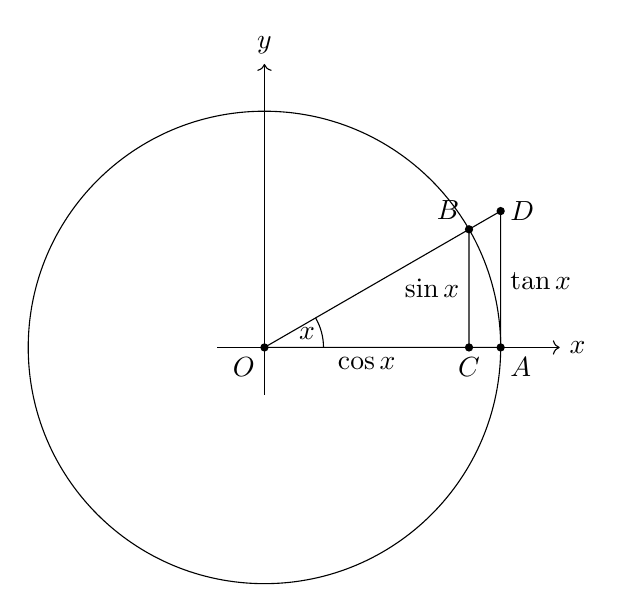
\begin{tikzpicture}[scale=3]
\coordinate (O) at (0,0);
\coordinate (A) at (1,0);
\coordinate (B) at ({cos(30)},{sin(30)});
\coordinate (C) at ({cos(30)},0);
\coordinate (D) at (1,{tan(30)});
\draw[->] (-0.2,0) -- (1.25,0) node[right] {$x$};
\draw[->] (0,-0.2) -- (0,1.2) node[above] {$y$};
\draw (O) circle (1);
\draw (O)--(A) (O)--(D) (B)--(C) (A)--(D);
\fill (O) circle (0.5pt) node[below left] {$O$};
\fill (A) circle (0.5pt) node[below right] {$A$};
\fill (B) circle (0.5pt) node[above left] {$B$};
\fill (C) circle (0.5pt) node[below] {$C$};
\fill (D) circle (0.5pt) node[right] {$D$};
\draw (0.25,0) arc (0:30:0.25);
\node at (0.18,0.06) {$x$};
\node[right] at (1,0.28) {$\tan x$};
\node[left] at ({cos(30)},0.25) {$\sin x$};
\node[below] at ({cos(30)/2},0) {$\cos x$};
\end{tikzpicture}
\end{center}
% SOURCE-END U0028
% PRESENTATION-SCAFFOLD close continued environment
\end{custom}
}
\end{frame}
% FRAME-ID F028
\begin{frame}[t,fragile]{两个重要极限（续2）}
\small
{\small
% REPEATED-CONTEXT environment continuation
\begin{custom}{几何直观：从单位圆看起}
% SOURCE-BEGIN U0028 915 1242


图中：
\begin{itemize}
\item 角 \(x\) 对应的圆弧长 = \(x\)（因为半径=1，弧长=半径×角度）
\item 垂线 \(BC\) 的长度 = \(\sin x\)
\item 水平线 \(OC\) 的长度 = \(\cos x\)
\item 切线 \(AD\) 的长度 = \(\tan x\)
\end{itemize}

从图中可以看出，三个面积之间有如下关系：

\[
\triangle OAB \text{ 的面积 } < \text{ 扇形 } OAB \text{ 的面积 } < \triangle OAD \text{ 的面积}.
\]

\end{custom}
% SOURCE-END U0028
}
\end{frame}
% FRAME-ID F029
\begin{frame}[t,fragile]{两个重要极限}
\small
{\small
% SOURCE-BEGIN U0029 0 491
\begin{custom}{面积比较}

\begin{itemize}
\item \(\triangle OAB\) 的面积 = \(\dfrac{1}{2} \times 1 \times \sin x = \dfrac{1}{2} \sin x\)
\item 扇形 \(OAB\) 的面积 = \(\dfrac{1}{2} \times 1^2 \times x = \dfrac{x}{2}\)
\item \(\triangle OAD\) 的面积 = \(\dfrac{1}{2} \times 1 \times \tan x = \dfrac{1}{2} \tan x\)
\end{itemize}

因此：

\[
\dfrac{1}{2} \sin x  <  \dfrac{x}{2} < \dfrac{1}{2} \tan x \qquad (0 < x < \dfrac{\pi}{2}).
\]

两边同时乘以 2，得到：

\[
\sin x  < x < \tan x.
\]

\end{custom}
% SOURCE-END U0029
}
\end{frame}
% FRAME-ID F030
\begin{frame}[t,fragile]{两个重要极限}
\footnotesize
{\footnotesize
% SOURCE-BEGIN U0030 0 394
\begin{custom}{推导 \(\dfrac{\sin x}{x}\) 的夹逼不等式}

由 \(x < \tan x = \dfrac{\sin x}{\cos x}\)，两边同时除以 \(\sin x > 0\)，得：

\[
\dfrac{x}{\sin x} < \dfrac{1}{\cos x} \quad \Longrightarrow \quad \cos x < \dfrac{\sin x}{x}.
\]

又由 \(\sin x < x\)，两边除以 \(x > 0\)，得：

\[
\dfrac{\sin x}{x} < 1.
\]

合起来：

\[
\cos x < \dfrac{\sin x}{x} < 1 \qquad (0 < x < \dfrac{\pi}{2}).
\]

\end{custom}
% SOURCE-END U0030
}
\end{frame}
% FRAME-ID F031
\begin{frame}[t,fragile]{两个重要极限}
\footnotesize
{\footnotesize
% SOURCE-BEGIN U0031 0 425
\begin{custom}{用夹逼准则取极限}

由 \(|\sin u|\leq|u|\)，有
\[
0\leq1-\cos x=2\sin^2\frac x2\leq\frac{x^2}{2},
\]
所以由夹逼定理可先得到 \(\lim_{x\to0}\cos x=1\)。因此，当 \(x \to 0^+\) 时：

\[
\cos x \;\longrightarrow\; 1,\quad \dfrac{\sin x}{x} \;\longrightarrow\; 1.
\]

当 \(x\) 为负时（即 \(x \to 0^-\)），由于 \(\dfrac{\sin x}{x}\) 是偶函数（\(\sin(-x)/(-x) = \sin x / x\)），左右极限相等。因此：

\[
\lim_{x \to 0} \dfrac{\sin x}{x} = 1.
\]

\end{custom}
% SOURCE-END U0031
}
\end{frame}
% FRAME-ID F032
\begin{frame}[t,fragile]{两个重要极限}
\normalsize
\begin{block}{例题}
{\normalsize
% SOURCE-BEGIN U0032 0 42
求 \(\lim_{x \to 0} \dfrac{\sin 2x}{x}\)。

% SOURCE-END U0032
}
\end{block}
\pause
{\normalsize
\textbf{解：}
% SOURCE-BEGIN U0033 0 79
\[
	\dfrac{\sin 2x}{x} = 2 \cdot \dfrac{\sin 2x}{2x} \to 2 \cdot 1 = 2.
	\]

% SOURCE-END U0033
}
\end{frame}
% FRAME-ID F033
\begin{frame}[t,fragile]{两个重要极限}
\small
{\small
% SOURCE-BEGIN U0034 0 427
\begin{application}[物理：小角度近似]

这个极限告诉我们：当角度 \(x\) 非常小时，\(\sin x\) 和 \(x\) 几乎相等。这里的角度必须使用\textbf{弧度}。例如：

\[
x = 0.1 \text{ 弧度} \approx 5.73^\circ,\quad \sin(0.1) \approx 0.099833,\quad \dfrac{\sin 0.1}{0.1} \approx 0.99833.
\]

\[
x = 0.01 \text{ 弧度},\quad \dfrac{\sin 0.01}{0.01} \approx 0.999983.
\]

误差非常小，且随 \(x\) 越小，比值越接近 $1$。这一近似常见于小振幅单摆、光学近轴近似和小角度机械运动。本章只由极限说明近似成立，不提前使用泰勒公式；第6章将进一步估计误差。

\end{application}
% SOURCE-END U0034
}
\end{frame}
% FRAME-ID F034
\begin{frame}[t,fragile]{两个重要极限}
\footnotesize
{\footnotesize
% SOURCE-BEGIN U0035 0 416
\begin{application}[生物医学：饱和响应的低浓度近似]
设教学模型
\[
v(C)=\frac{V_{\max}C}{K+C},\qquad V_{\max}>0,\quad K>0,
\]
其中 $C$ 表示浓度，$v(C)$ 表示响应速率。假设在所研究范围内参数保持不变，则
\[
\frac{v(C)}{C}=\frac{V_{\max}}{K+C}
\longrightarrow\frac{V_{\max}}K
\qquad(C\to0^+).
\]
因此在低浓度范围内，
\[
v(C)\approx\frac{V_{\max}}K\,C.
\]
这说明非线性响应在局部可以近似为线性。本例只用于展示局部近似结构，不应把该公式直接解释为临床剂量关系；具体生物系统还可能存在多种反应途径和参数变化。\upcite{NCBIEnzyme}
\end{application}
% SOURCE-END U0035
}
\end{frame}
% FRAME-ID F035
\begin{frame}[t,fragile]{两个重要极限}
\normalsize
{\normalsize
% SOURCE-BEGIN U0036 0 28
\subsubsection*{第二个重要极限}


% SOURCE-END U0036
}
\end{frame}
% FRAME-ID F036
\begin{frame}[t,fragile]{两个重要极限}
\normalsize
\begin{block}{定理}
{\normalsize
% SOURCE-BEGIN U0037 0 92
\textbf{自然常数 e }\par

	\[
	\lim_{n\to\infty} \left(1 + \dfrac{1}{n}\right)^n = \ee.
	\]

% SOURCE-END U0037
}
\end{block}
\end{frame}
% FRAME-ID F037
\begin{frame}[t,fragile]{两个重要极限}
\footnotesize
{\footnotesize
% SOURCE-BEGIN U0038 0 692
\begin{custom}{具体证明}
	证明分为两步：先证 \(\{a_n\}\) 单调递增，再证它有上界。
	
	\noindent\textbf{第一步：证明单调递增}
	
	由二项式定理展开：
	\[
	a_n = \left(1+\dfrac{1}{n}\right)^n = \sum\limits_{k=0}^{n} C_n^k \dfrac{1}{n^k} = \sum_{k=0}^{n} \dfrac{1}{k!} \cdot \dfrac{n(n-1)\cdots(n-k+1)}{n^k}.
	\]
	其中 \(\dfrac{n(n-1)\cdots(n-k+1)}{n^k} = 1 \cdot \left(1-\dfrac{1}{n}\right) \cdots \left(1-\dfrac{k-1}{n}\right)\)。于是
	\[
	a_n = \sum_{k=0}^{n} \dfrac{1}{k!} \left(1-\dfrac{1}{n}\right)\left(1-\dfrac{2}{n}\right)\cdots\left(1-\dfrac{k-1}{n}\right).
	\]
	
	同理，
	\[
	a_{n+1} = \sum_{k=0}^{n+1} \dfrac{1}{k!} \left(1-\dfrac{1}{n+1}\right)\left(1-\dfrac{2}{n+1}\right)\cdots\left(1-\dfrac{k-1}{n+1}\right).
	\]
	

% SOURCE-END U0038
% PRESENTATION-SCAFFOLD close continued environment
\end{custom}
}
\end{frame}
% FRAME-ID F038
\begin{frame}[t,fragile]{两个重要极限（续1）}
\small
{\small
% REPEATED-CONTEXT environment continuation
\begin{custom}{具体证明}
% SOURCE-BEGIN U0038 692 1277
	比较 \(a_n\) 与 \(a_{n+1}\) 中 \(k\) 相同的项（\(1 \leq k \leq n\)）：
	\[
	\left(1-\dfrac{1}{n}\right)\left(1-\dfrac{2}{n}\right)\cdots\left(1-\dfrac{k-1}{n}\right) < \left(1-\dfrac{1}{n+1}\right)\left(1-\dfrac{2}{n+1}\right)\cdots\left(1-\dfrac{k-1}{n+1}\right),
	\]
	因为每个因子 \(1-\dfrac{j}{n}<1-\dfrac{j}{n+1}\)（\(j=1,2,\dots,k-1\)），并且 \(a_{n+1}\) 还多出一个正项。因此
	\[
	a_n < a_{n+1},
	\]
	故数列严格递增。
	
	\noindent\textbf{第二步：证明有上界}
	
	由展开式，
	\[
	a_n = \sum_{k=0}^{n} \dfrac{1}{k!} \left(1-\dfrac{1}{n}\right)\cdots\left(1-\dfrac{k-1}{n}\right) \leq \sum_{k=0}^{n} \dfrac{1}{k!}.
	\]
	

% SOURCE-END U0038
% PRESENTATION-SCAFFOLD close continued environment
\end{custom}
}
\end{frame}
% FRAME-ID F039
\begin{frame}[t,fragile]{两个重要极限（续2）}
\footnotesize
{\footnotesize
% REPEATED-CONTEXT environment continuation
\begin{custom}{具体证明}
% SOURCE-BEGIN U0038 1277 1818
	当 \(k \geq 1\) 时，\(k! = 1 \cdot 2 \cdot 3 \cdots k \geq 1 \cdot 2 \cdot 2 \cdots 2 = 2^{k-1}\)，因此
	\[
	\dfrac{1}{k!} \leq \dfrac{1}{2^{k-1}} \quad (k \geq 1).
	\]
	
	于是
	\[
	a_n < 1 + 1 + \dfrac{1}{2} + \dfrac{1}{2^2} + \cdots + \dfrac{1}{2^{n-1}} = 1 + \dfrac{1 - (1/2)^n}{1 - 1/2} = 1 + 2\left(1 - \dfrac{1}{2^n}\right) < 3.
	\]
	
	所以 \(a_n < 3\) 对所有 \(n\) 成立，数列有上界。
	
	\noindent\textbf{结论：} 数列 \(\{a_n\}\) 单调递增且有上界，由单调有界准则，极限存在。记这个极限为 \(\ee\)，即
	\[
	\ee = \lim_{n\to\infty} \left(1+\dfrac{1}{n}\right)^n.
	\]
\end{custom}
% SOURCE-END U0038
}
\end{frame}
% FRAME-ID F040
\begin{frame}[t,fragile]{两个重要极限}
\normalsize
\begin{block}{定理}
{\normalsize
% SOURCE-BEGIN U0039 0 61
\textbf{第二个重要极限}\par

\[
\lim_{x\to0}(1+x)^{1/x}=\ee.
\]

% SOURCE-END U0039
}
\end{block}
\end{frame}
% FRAME-ID F041
\begin{frame}[t,fragile]{两个重要极限}
\footnotesize
{\footnotesize
\textbf{证明：}
% SOURCE-BEGIN U0040 0 517
先考虑 \(x\to0^+\)。令
\[
n=\left\lfloor\frac1x\right\rfloor,
\]
则当 \(x\to0^+\) 时 \(n\to\infty\)，并且
\[
\frac1{n+1}<x\leq\frac1n,\qquad n\leq\frac1x<n+1.
\]
由于此时各底数都大于 \(1\)，有
\[
\left(1+\frac1{n+1}\right)^n
\leq(1+x)^{1/x}
\leq\left(1+\frac1n\right)^{n+1}.
\]
记 \(a_n=(1+\frac1n)^n\)。前面已经证明 \(a_n\to\ee\)，而
\[
\left(1+\frac1{n+1}\right)^n
=\frac{a_{n+1}}{1+\frac1{n+1}}\to\ee,
\]
\[
\left(1+\frac1n\right)^{n+1}
=a_n\left(1+\frac1n\right)\to\ee.
\]
由夹逼定理，
\[
\lim_{x\to0^+}(1+x)^{1/x}=\ee.
\]


% SOURCE-END U0040
}
\end{frame}
% FRAME-ID F042
\begin{frame}[t,fragile]{两个重要极限（续1）}
\normalsize
{\normalsize
\textbf{证明：}
% SOURCE-BEGIN U0040 517 763
再考虑 \(x\to0^-\)。当 \(x\) 充分接近 \(0\) 时 \(x>-1\)。令
\[
y=-\frac{x}{1+x},
\]
则 \(y\to0^+\)，且 \(1+x=(1+y)^{-1}\)、\(1/x=-(1+y)/y\)。因此
\[
(1+x)^{1/x}
=(1+y)^{(1+y)/y}
=(1+y)^{1/y}(1+y)\to\ee.
\]
左右极限相等，所以
\[
\lim_{x\to0}(1+x)^{1/x}=\ee.
\]

% SOURCE-END U0040
}
\end{frame}
% FRAME-ID F043
\begin{frame}[t,fragile]{两个重要极限}
\normalsize
\begin{block}{定理}
{\normalsize
% SOURCE-BEGIN U0041 0 101
\textbf{第二个重要极限的离散推广}\par

对任意实数 \(a\)，
\[
\lim_{n\to\infty}\left(1+\frac an\right)^n=\ee^a.
\]

% SOURCE-END U0041
}
\end{block}
\pause
{\normalsize
\textbf{证明：}
% SOURCE-BEGIN U0042 0 171
当 \(a=0\) 时结论显然成立。当 \(a\neq0\) 时，令 \(x=a/n\)，则 \(x\to0\)，且对充分大的 \(n\)，\(1+a/n>0\)。于是
\[
\left(1+\frac an\right)^n
=\left[(1+x)^{1/x}\right]^a\longrightarrow\ee^a.
\]

% SOURCE-END U0042
}
\end{frame}
% FRAME-ID F044
\begin{frame}[t,fragile]{两个重要极限}
\normalsize
\begin{block}{例题}
{\normalsize
% SOURCE-BEGIN U0043 0 65
求 \(\lim\limits_{n\to\infty} \left(1 + \dfrac{2}{n}\right)^n\)。

% SOURCE-END U0043
}
\end{block}
\pause
{\normalsize
\textbf{解：}
% SOURCE-BEGIN U0044 0 109
\[
	\left(1 + \dfrac{2}{n}\right)^n = \left[\left(1 + \dfrac{1}{n/2}\right)^{n/2}\right]^2 \to \ee^2.
	\]

% SOURCE-END U0044
}
\end{frame}
\section{等价无穷小}
% FRAME-ID F045
\begin{frame}[t,fragile]{目录}
\normalsize
{\color{black}\normalsize 1. 一元函数极限\par}\vspace{0.22em}
{\color{black}\normalsize 2. 函数极限的基本性质\par}\vspace{0.22em}
{\color{black}\normalsize 3. 两个重要极限\par}\vspace{0.22em}
{\color{blue}\normalsize 4. 等价无穷小\par}\vspace{0.22em}
{\color{gray!40}\normalsize 5. 一元函数的连续性\par}\vspace{0.22em}
{\color{gray!40}\normalsize 6. 闭区间连续函数的两个基本定理\par}\vspace{0.22em}
{\color{gray!40}\normalsize 7. 二元函数的极限与连续\par}\vspace{0.22em}
\end{frame}
% FRAME-ID F046
\begin{frame}[t,fragile]{等价无穷小}
\normalsize
{\normalsize
% SOURCE-BEGIN U0045 0 75
在计算极限时，我们经常遇到两个无穷小量相乘或相除的情况。如果能用一个简单的无穷小量代替复杂的无穷小量，计算会大大简化。这就是等价无穷小的思想。


% SOURCE-END U0045
}
\end{frame}
% FRAME-ID F047
\begin{frame}[t,fragile]{等价无穷小}
\normalsize
\begin{block}{定义}
{\normalsize
% SOURCE-BEGIN U0046 0 461
\textbf{无穷小量}\par

	如果 $\lim _{x \rightarrow a} f(x)=0$ ，那么 $f(x)$ 称为是 $x \rightarrow a$ 时的无穷小量．如果 $f(x)$ 与 $g(x)$都是 $x \rightarrow a$ 时的无穷小量，那么
	\begin{itemize}
		\item[1．] 当 $\lim _{x \rightarrow a} \frac{g(x)}{f(x)}=0$ 时，说 $g(x)$ 是 $f(x)$ 的高阶无穷小，记为 $g(x)=o(f(x))$ ；
		\item[2．] 当 $\lim _{x \rightarrow a} \frac{g(x)}{f(x)}=L>0$ 时，说 $g(x)$ 是 $f(x)$ 的同阶无穷小，特别地，当 $L=1$ 时，称为等价无穷小，记为 $\mathrm{f}(\mathrm{x}) \sim \mathrm{g}(\mathrm{x})$ ；
	\end{itemize}


% SOURCE-END U0046
}
\end{block}
\end{frame}
% FRAME-ID F048
\begin{frame}[t,fragile]{等价无穷小}
\normalsize
{\normalsize
% SOURCE-BEGIN U0047 0 78
\subsubsection{\texorpdfstring{常用等价无穷小（\(x \to 0\) 时）}{常用等价无穷小（x 趋于 0 时）}}


% SOURCE-END U0047
}
{\normalsize
% SOURCE-BEGIN U0048 0 25
以下等价关系是微积分中最常用的，务必熟记：


% SOURCE-END U0048
}
{\normalsize
% SOURCE-BEGIN U0049 0 246
\[
\boxed{
\begin{aligned}
\sin x &\sim x & \tan x &\sim x \\
\arcsin x &\sim x & \arctan x &\sim x \\
\ee^x - 1 &\sim x & \ln(1+x) &\sim x \\
1 - \cos x &\sim \dfrac{x^2}{2} & (1+x)^a - 1 &\sim ax \quad (a \neq 0)
\end{aligned}
}
\]


% SOURCE-END U0049
}
\end{frame}
% FRAME-ID F049
\begin{frame}[t,fragile]{等价无穷小}
\normalsize
{\normalsize
% SOURCE-BEGIN U0050 0 100
本章在处理指数、对数和三角函数时，使用高中阶段已经熟悉的初等函数基本连续性，例如 $\ln x$ 在 $x>0$ 上连续。本章后半部分将用极限语言正式定义函数连续性，并系统讨论一般连续函数的性质。

% SOURCE-END U0050
}
\end{frame}
% FRAME-ID F050
\begin{frame}[t,fragile]{等价无穷小}
\small
{\small
% SOURCE-BEGIN U0051 0 445
\begin{custom}{几个等价关系的推导}

\begin{itemize}
\item \textbf{\(\sin x \sim x\)：} 这就是我们之前证明的 \(\lim_{x \to 0} \dfrac{\sin x}{x} = 1\)。

\item \textbf{\(\tan x \sim x\)：} 
\[
\lim_{x \to 0} \dfrac{\tan x}{x} = \lim_{x \to 0} \dfrac{\sin x}{x} \cdot \dfrac{1}{\cos x} = 1 \cdot 1 = 1.
\]

\item \textbf{\(\ln(1+x)\sim x\)：} 由第二个重要极限及对数函数的连续性，
\[
\lim_{x\to0}\frac{\ln(1+x)}{x}
=\lim_{x\to0}\ln\!\left[(1+x)^{1/x}\right]
=\ln\ee=1.
\]


% SOURCE-END U0051
% PRESENTATION-SCAFFOLD close continued environment
\end{itemize}\end{custom}
}
\end{frame}
% FRAME-ID F051
\begin{frame}[t,fragile]{等价无穷小（续1）}
\footnotesize
{\footnotesize
% REPEATED-CONTEXT environment continuation
\begin{custom}{几个等价关系的推导}

\begin{itemize}

% SOURCE-BEGIN U0051 445 1142
\item \textbf{\(\ee^x-1\sim x\)：} 令 \(t=\ee^x-1\)，则 \(x=\ln(1+t)\)。当 \(x\to0\) 时 \(t\to0\)，利用刚证明的 \(\ln(1+t)\sim t\)，
\[
\lim_{x\to0}\frac{\ee^x-1}{x}
=\lim_{t\to0}\frac{t}{\ln(1+t)}=1.
\]

\item \textbf{\(1 - \cos x \sim \dfrac{x^2}{2}\)：} 
\[
\lim_{x \to 0} \dfrac{1 - \cos x}{x^2/2} = \lim_{x \to 0} \dfrac{2 \sin^2(x/2)}{x^2/2} = \lim_{x \to 0} \dfrac{4 \sin^2(x/2)}{x^2} = \lim_{x \to 0} \left(\dfrac{\sin(x/2)}{x/2}\right)^2 = 1.
\]

\item \textbf{\((1+x)^a - 1 \sim ax\)：} 
\[
\lim_{x \to 0} \dfrac{(1+x)^a - 1}{ax} = \dfrac{1}{a} \cdot \lim_{x \to 0} \dfrac{\ee^{a\ln(1+x)} - 1}{x} = \dfrac{1}{a} \cdot \lim_{x \to 0} \dfrac{a\ln(1+x)}{x} = 1.
\]
\end{itemize}
\end{custom}
% SOURCE-END U0051
}
\end{frame}
% FRAME-ID F052
\begin{frame}[t,fragile]{等价无穷小}
\normalsize
{\normalsize
% SOURCE-BEGIN U0052 0 35
\subsubsection{等价无穷小的应用：简化极限计算}


% SOURCE-END U0052
}
\end{frame}
% FRAME-ID F053
\begin{frame}[t,fragile]{等价无穷小}
\normalsize
{\normalsize
% SOURCE-BEGIN U0053 0 238
\begin{custom}{核心原则}
在乘除结构中，可以用等价无穷小替换来简化计算：
\[
\lim \dfrac{f(x)}{g(x)} = \lim \dfrac{\tilde{f}(x)}{\tilde{g}(x)},
\]
其中 \(\tilde{f} \sim f\)，\(\tilde{g} \sim g\)。

\textbf{但注意：} 在加减结构中，不能随意替换！因为主要项可能相互抵消，替换后可能丢失关键信息。
\end{custom}
% SOURCE-END U0053
}
\end{frame}
% FRAME-ID F054
\begin{frame}[t,fragile]{等价无穷小}
\normalsize
\begin{block}{例题}
{\normalsize
% SOURCE-BEGIN U0054 0 91
\textbf{乘除结构中的替换}\par

求 \(\lim\limits_{x \to 0} \dfrac{\sin 2x \cdot \ln(1+3x)}{x^2}\)。

% SOURCE-END U0054
}
\end{block}
\pause
{\normalsize
\textbf{解：}
% SOURCE-BEGIN U0055 0 351
当 \(x \to 0\) 时，\(\sin 2x \sim 2x\)，\(\ln(1+3x) \sim 3x\)，所以
\[
\dfrac{\sin 2x \cdot \ln(1+3x)}{x^2} \sim \dfrac{(2x) \cdot (3x)}{x^2} = 6 \quad \Rightarrow \quad \text{极限为 } 6.
\]
更严谨地：
\[
\lim_{x \to 0} \dfrac{\sin 2x \cdot \ln(1+3x)}{x^2} = \lim_{x \to 0} \dfrac{\sin 2x}{2x} \cdot \dfrac{\ln(1+3x)}{3x} \cdot 6 = 1 \cdot 1 \cdot 6 = 6.
\]

% SOURCE-END U0055
}
\end{frame}
% FRAME-ID F055
\begin{frame}[t,fragile]{等价无穷小}
\normalsize
\begin{block}{例题}
{\normalsize
% SOURCE-BEGIN U0056 0 85
\textbf{加减结构的拆分}\par

求 \(\lim\limits_{x \to 0} \dfrac{\ee^{x^2} - \cos x}{x^2}\)。

% SOURCE-END U0056
}
\end{block}
\pause
{\normalsize
\textbf{解：}
% SOURCE-BEGIN U0057 0 372
这里分子是两项相减，不能把 \(\ee^{x^2}\) 与 \(\cos x\) 都直接替换为 \(1\)。将分子按已知等价无穷小拆分：
\[
\frac{\ee^{x^2}-\cos x}{x^2}
=\frac{\ee^{x^2}-1}{x^2}+\frac{1-\cos x}{x^2}.
\]
由于 \(\ee^u-1\sim u\)（取 \(u=x^2\)）且 \(1-\cos x\sim x^2/2\)，所以
\[
\lim_{x\to0}\frac{\ee^{x^2}-\cos x}{x^2}
=1+\frac12=\frac32.
\]

\textbf{注意：} 这里不能直接用 \(\ee^{x^2}\sim1\) 和 \(\cos x\sim1\)，因为 \(1-1=0\) 会丢失主要信息。

% SOURCE-END U0057
}
\end{frame}
% FRAME-ID F056
\begin{frame}[t,fragile]{等价无穷小}
\footnotesize
\begin{block}{例题}
{\footnotesize
% SOURCE-BEGIN U0058 0 672
\textbf{加减结构中的易错点}\par

求 \(\lim\limits_{x \to 0} \dfrac{\tan x - \sin x}{x^3}\)。




\begin{solution}
	先用恒等变形把相减结构改写为乘除结构：
	\[
	\frac{\tan x-\sin x}{x^3}
	=\frac{\sin x(1-\cos x)}{x^3\cos x}.
	\]
	利用 \(\sin x\sim x\)、\(1-\cos x\sim x^2/2\) 以及 \(\cos x\to1\)，得到
	\[
	\lim_{x\to0}\frac{\tan x-\sin x}{x^3}
	=\frac12.
	\]
	
\end{solution}

\textbf{注意：} 这里不能直接使用 \(\tan x \sim x\)，\(\sin x \sim x\)，否则 \(\tan x - \sin x \sim x - x = 0\)，极限为 0。


\iffalse

\begin{custom}{后续方法预告}
学习泰勒公式后，也可以写成
\[
\tan x=x+\frac{x^3}{3}+o(x^3),\qquad
\sin x=x-\frac{x^3}{6}+o(x^3),
\]
从而立即看出三次项的系数之差为 \(1/2\)。这里仅作方法预告，不把尚未建立的泰勒公式作为当前证明的依据。
\end{custom}

\fi

% SOURCE-END U0058
}
\end{block}
\end{frame}
% FRAME-ID F057
\begin{frame}[t,fragile]{等价无穷小}
\footnotesize
{\footnotesize
% SOURCE-BEGIN U0059 0 608
\begin{custom}{等价无穷小替换的口诀}
\begin{center}
\fbox{\parbox{0.85\textwidth}{
\textbf{乘除可换因子，加减先防抵消。}\\
\textbf{当前先作恒等变形，学完泰勒公式后再看高阶项。}}
}
\end{center}

\textbf{具体规则：}
\begin{itemize}
\item 在乘除结构中：可以用等价无穷小替换因子。
\item 在加减结构中，不能仅由 $\alpha\sim\widetilde\alpha$、$\beta\sim\widetilde\beta$ 就把各项分别替换后再相加或相减，因为主项可能发生抵消。
\item 若已经证明 $\alpha=o(\beta)$，则
\[
\alpha+\beta
=\beta\left(1+\frac{\alpha}{\beta}\right)
=\beta[1+o(1)]
\sim\beta.
\]
此时可以说高阶项 $\alpha$ 相对于主项 $\beta$ 可以忽略。
\item 若两个无穷小同阶，尤其需要警惕主项抵消；若发生抵消，应使用恒等变形、已知极限或后续的泰勒展开继续分析。“不是同阶”本身也不保证存在明确的高阶关系，例如两个无穷小的比值可能振荡。
\end{itemize}
\end{custom}
% SOURCE-END U0059
}
\end{frame}
% FRAME-ID F058
\begin{frame}[t,fragile]{等价无穷小}
\normalsize
{\normalsize
% SOURCE-BEGIN U0060 0 34
\subsubsection{等价无穷小与无穷小量阶的比较}


% SOURCE-END U0060
}
{\normalsize
% SOURCE-BEGIN U0061 0 37
为了更精确地描述无穷小量趋近于 0 的“速度”，我们引入阶的概念。


% SOURCE-END U0061
}
\end{frame}
% FRAME-ID F059
\begin{frame}[t,fragile]{等价无穷小}
\normalsize
\begin{block}{定义}
{\normalsize
% SOURCE-BEGIN U0062 0 386
\textbf{无穷小的阶}\par

设 \(\alpha(x) \to 0\)，\(\beta(x) \to 0\)，且 \(\beta(x) \neq 0\)。
\begin{itemize}
\item 若 \(\lim \dfrac{\alpha}{\beta} = 0\)，称 \(\alpha\) 是比 \(\beta\) 高阶的无穷小，记作 \(\alpha = o(\beta)\)。
\item 若 \(\lim \dfrac{\alpha}{\beta} = C \neq 0\)，称 \(\alpha\) 与 \(\beta\) 是同阶无穷小。
\item 特别地，若 \(C = 1\)，称 \(\alpha\) 与 \(\beta\) 是等价无穷小，记作 \(\alpha \sim \beta\)。
\end{itemize}

% SOURCE-END U0062
}
\end{block}
\end{frame}
% FRAME-ID F060
\begin{frame}[t,fragile]{等价无穷小}
\normalsize
{\normalsize
% SOURCE-BEGIN U0063 0 488
\begin{custom}{阶的比较：举例}
当 \(x \to 0\) 时：
\begin{itemize}
\item \(x^2\) 是比 \(x\) 高阶的无穷小：\(\dfrac{x^2}{x} = x \to 0\)，记作 \(x^2 = o(x)\)。
\item \(x^2\) 与 \(2x^2\) 是同阶无穷小：\(\dfrac{x^2}{2x^2} = \dfrac{1}{2}\)。
\item \(x\) 与 \(\sin x\) 是等价无穷小：\(\dfrac{x}{\sin x} \to 1\)。
\end{itemize}

\textbf{阶的比较示意图：}
\[
\underbrace{x^3}_{o(x^2)} \quad \ll \quad \underbrace{x^2}_{o(x)} \quad \ll \quad \underbrace{x}_{\text{一阶}} \quad \ll \quad \underbrace{\sqrt{x}}_{\text{低阶}}
\]
\end{custom}
% SOURCE-END U0063
}
\end{frame}
% FRAME-ID F061
\begin{frame}[t,fragile]{等价无穷小}
\footnotesize
{\footnotesize
% SOURCE-BEGIN U0065 0 530
\begin{extra}
\subsection*{等价无穷小的推广（选读）}


\begin{custom}{推广一：复合函数的等价替换}
若当 \(u \to 0\) 时 \(f(u) \sim g(u)\)，且 \(u(x) \to 0\)，则当 \(x \to x_0\) 时 \(f(u(x)) \sim g(u(x))\)。

例如：\(\sin(x^2) \sim x^2\)（因为 \(x^2 \to 0\)），\(\ln(1+\sin x) \sim \sin x \sim x\)。

\begin{example}
求 \(\lim\limits_{x \to 0} \dfrac{\ln(1 + \sin x)}{x}\)。
\end{example}
\begin{solution}
当 \(x \to 0\) 时，\(\sin x \to 0\)，所以 \(\ln(1+\sin x) \sim \sin x \sim x\)，因此
\[
\lim_{x \to 0} \dfrac{\ln(1+\sin x)}{x} = 1.
\]
\end{solution}
\end{custom}
% SOURCE-END U0065
% PRESENTATION-SCAFFOLD close continued environment
\end{extra}
}
\end{frame}
% FRAME-ID F062
\begin{frame}[t,fragile]{等价无穷小（续1）}
\normalsize
{\normalsize
% REPEATED-CONTEXT environment continuation
\begin{extra}

% SOURCE-BEGIN U0065 530 749


\begin{custom}{推广二：多个等价无穷小的链式替换}
若 \(\alpha \sim \beta\)，\(\beta \sim \gamma\)，则 \(\alpha \sim \gamma\)。等价关系具有传递性。

例如：\(\ee^x - 1 \sim x \sim \ln(1+x)\)，所以 \(\ee^x - 1 \sim \ln(1+x)\)。
\end{custom}
\end{extra}
% SOURCE-END U0065
}
\end{frame}
% FRAME-ID F063
\begin{frame}[t,fragile]{等价无穷小}
\normalsize
{\normalsize
% SOURCE-BEGIN U0067 0 464
\begin{extra}
\subsection*{Stolz定理（选读）}

Stolz定理可以看作处理某些 \(\dfrac{\infty}{\infty}\) 型数列极限的离散版洛必达法则：
设 \(\{a_n\}, \{b_n\}\) 满足 \(b_n \to +\infty\) 且单调递增，若 \(\lim \dfrac{a_{n+1}-a_n}{b_{n+1}-b_n} = L\)，则 \(\lim \dfrac{a_n}{b_n} = L\)。

例如，用Stolz定理可证 \(\lim_{n\to\infty} \dfrac{\ln n}{n} = 0\)：
\[
\lim_{n\to\infty} \dfrac{\ln n}{n} = \lim_{n\to\infty} \dfrac{\ln(n+1) - \ln n}{(n+1)-n} = \lim_{n\to\infty} \ln\left(1+\dfrac{1}{n}\right) = 0.
\]
\end{extra}
% SOURCE-END U0067
}
\end{frame}
\section{一元函数的连续性}
% FRAME-ID F064
\begin{frame}[t,fragile]{目录}
\normalsize
{\color{black}\normalsize 1. 一元函数极限\par}\vspace{0.22em}
{\color{black}\normalsize 2. 函数极限的基本性质\par}\vspace{0.22em}
{\color{black}\normalsize 3. 两个重要极限\par}\vspace{0.22em}
{\color{black}\normalsize 4. 等价无穷小\par}\vspace{0.22em}
{\color{blue}\normalsize 5. 一元函数的连续性\par}\vspace{0.22em}
{\color{gray!40}\normalsize 6. 闭区间连续函数的两个基本定理\par}\vspace{0.22em}
{\color{gray!40}\normalsize 7. 二元函数的极限与连续\par}\vspace{0.22em}
\end{frame}
% FRAME-ID F065
\begin{frame}[t,fragile]{一元函数的连续性}
\normalsize
\begin{block}{定义}
{\normalsize
% SOURCE-BEGIN U0068 0 240
\textbf{函数在一点连续}\par

设函数 $f$ 在点 $x_0$ 的某邻域内有定义，且 $f(x_0)$ 有定义。 若
\[
\lim_{x\to x_0}f(x)=f(x_0),
\]
则称 $f$ 在点 $x_0$ 处连续。 等价地，对任意 $\varepsilon>0$，存在 $\delta>0$，使得当 $|x-x_0|<\delta$ 且 $x$ 属于函数定义域时，都有
\[
|f(x)-f(x_0)|<\varepsilon.
\]

% SOURCE-END U0068
}
\end{block}
\end{frame}
% FRAME-ID F066
\begin{frame}[t,fragile]{一元函数的连续性}
\normalsize
\begin{block}{定义}
{\normalsize
% SOURCE-BEGIN U0069 0 179
\textbf{左右连续}\par

若
\[
\lim_{x\to x_0-}f(x)=f(x_0),
\]
则称 $f$ 在 $x_0$ 处左连续；若
\[
\lim_{x\to x_0+}f(x)=f(x_0),
\]
则称 $f$ 在 $x_0$ 处右连续。 函数在 $x_0$ 连续，当且仅当它在 $x_0$ 左连续且右连续。

% SOURCE-END U0069
}
\end{block}
\end{frame}
% FRAME-ID F067
\begin{frame}[t,fragile]{一元函数的连续性}
\normalsize
\begin{block}{定义}
{\normalsize
% SOURCE-BEGIN U0070 0 184
\textbf{区间上的连续}\par

若 $f$ 在开区间 $(a,b)$ 内每一点连续，则称 $f$ 在 $(a,b)$ 上连续。 若 $f$ 在 $(a,b)$ 内连续，且
\[
\lim_{x\to a+}f(x)=f(a),\qquad \lim_{x\to b-}f(x)=f(b),
\]
则称 $f$ 在闭区间 $[a,b]$ 上连续。

% SOURCE-END U0070
}
\end{block}
\end{frame}
% FRAME-ID F068
\begin{frame}[t,fragile]{一元函数的连续性}
\normalsize
{\normalsize
% PRESENTATION-SCAFFOLD isotropic coordinates; node font size unchanged
\tikzset{every picture/.append style={scale=0.75}}
% SOURCE-BEGIN U0071 0 813
\begin{center}
\begin{tikzpicture}[scale=0.9,>=Stealth]
  \draw[->] (-0.3,0)--(5.8,0) node[right] {$x$};
  \draw[->] (0,-0.3)--(0,3.2) node[above] {$y$};
  \draw[domain=0.3:5.2,smooth,variable=\x,thick] plot ({\x},{1.4+0.35*sin(80*\x)});
  \node at (2.9,-0.55) {连续图像：局部变化不会出现跳跃};
\end{tikzpicture}
\qquad
\begin{tikzpicture}[scale=0.9,>=Stealth]
  \draw[->] (-0.3,0)--(5.8,0) node[right] {$x$};
  \draw[->] (0,-0.3)--(0,3.2) node[above] {$y$};
  \draw[domain=0.3:2.65,smooth,variable=\x,thick] plot ({\x},{0.7+0.25*\x});
  \draw[domain=2.75:5.2,smooth,variable=\x,thick] plot ({\x},{1.8+0.12*(\x-3)^2});
  \filldraw[white] (2.7,1.375) circle (2.2pt);
  \draw (2.7,1.375) circle (2.2pt);
  \fill (2.7,1.81) circle (2.2pt);
  \node at (2.9,-0.55) {不连续图像：极限值与函数值不一致};
\end{tikzpicture}
\end{center}
% SOURCE-END U0071
}
\end{frame}
% FRAME-ID F069
\begin{frame}[t,fragile]{一元函数的连续性}
\small
\begin{block}{命题}
{\small
% SOURCE-BEGIN U0072 0 118
\textbf{四则运算}\par

若 $f,g$ 在 $x_0$ 处连续，则 $f+g,\,f-g,\,fg$ 在 $x_0$ 处连续。 若 $g(x_0)\neq0$，则 $\frac{f}{g}$ 在 $x_0$ 处连续。

% SOURCE-END U0072
}
\end{block}
\pause
{\small
\textbf{证明：}
% SOURCE-BEGIN U0073 0 334
以乘积为例。 由连续性得
\[
\lim_{x\to x_0}f(x)=f(x_0),\qquad \lim_{x\to x_0}g(x)=g(x_0).
\]
由极限乘法法则，
\[
\lim_{x\to x_0}f(x)g(x)=f(x_0)g(x_0),
\]
故 $fg$ 在 $x_0$ 连续。 加、减同理。 对商函数，由 $g(x_0)\neq0$ 且 $g$ 连续，存在 $x_0$ 的某邻域使 $g(x)\neq0$，于是商函数在该邻域有定义，并由极限商法则得
\[
\lim_{x\to x_0}\frac{f(x)}{g(x)}=\frac{f(x_0)}{g(x_0)}.
\]
故 $\frac{f}{g}$ 连续。

% SOURCE-END U0073
}
\end{frame}
% FRAME-ID F070
\begin{frame}[t,fragile]{一元函数的连续性}
\small
\begin{block}{命题}
{\small
% SOURCE-BEGIN U0074 0 91
\textbf{复合函数连续性}\par

若 $g$ 在 $x_0$ 处连续，$f$ 在 $g(x_0)$ 处连续，则复合函数 $f\circ g$ 在 $x_0$ 处连续。

% SOURCE-END U0074
}
\end{block}
\pause
{\small
\textbf{证明：}
% SOURCE-BEGIN U0075 0 309
记 $y_0=g(x_0)$。 给定任意 $\varepsilon>0$。 因 $f$ 在 $y_0$ 处连续，存在 $\eta>0$，使得当 $|y-y_0|<\eta$ 时，
\[
|f(y)-f(y_0)|<\varepsilon.
\]
因 $g$ 在 $x_0$ 处连续，存在 $\delta>0$，使得当 $|x-x_0|<\delta$ 时，
\[
|g(x)-g(x_0)|<\eta.
\]
于是当 $|x-x_0|<\delta$ 时，
\[
|f(g(x))-f(g(x_0))|<\varepsilon.
\]
这正是 $f\circ g$ 在 $x_0$ 处连续。

% SOURCE-END U0075
}
\end{frame}
% FRAME-ID F071
\begin{frame}[t,fragile]{一元函数的连续性}
\normalsize
\begin{block}{定义}
{\normalsize
\setbeamertemplate{enumerate mini template}[default]
% SOURCE-BEGIN U0076 0 281
\textbf{间断点}\par

若 $f$ 在 $x_0$ 不连续，则称 $x_0$ 为 $f$ 的间断点。 常见情形包括：
\begin{enumerate}[(1)]
\item 可去间断：$\lim_{x\to x_0}f(x)$ 存在，但不等于 $f(x_0)$，或 $f(x_0)$ 未定义；
\item 跳跃间断：左右极限都存在但不相等；
\item 无穷间断：至少有一个单侧极限为 \(+\infty\) 或 \(-\infty\)；
\item 振荡间断：函数在该点附近无限振荡，极限不存在。
\end{enumerate}

% SOURCE-END U0076
}
\end{block}
\end{frame}
% FRAME-ID F072
\begin{frame}[t,fragile]{一元函数的连续性}
\normalsize
\begin{block}{例题}
{\normalsize
% SOURCE-BEGIN U0077 0 103
讨论函数
\[
f(x)=
\begin{cases}
\dfrac{\sin x}{x},&x\neq0,\\
a,&x=0
\end{cases}
\]
在 $x=0$ 处的连续性。

% SOURCE-END U0077
}
\end{block}
\pause
{\normalsize
\textbf{解：}
% SOURCE-BEGIN U0078 0 109
因为
\[
\lim_{x\to0}\frac{\sin x}{x}=1,
\]
所以 $f$ 在 $0$ 处连续当且仅当 $a=1$。 若 $a\neq1$，极限存在但不等于函数值，$0$ 是可去间断点。

% SOURCE-END U0078
}
\end{frame}
% FRAME-ID F073
\begin{frame}[t,fragile]{一元函数的连续性}
\normalsize
{\normalsize
% SOURCE-BEGIN U0079 0 78
\begin{warning}
分段函数在分段点处必须检查左极限、右极限和函数值三者。 只检查表达式能否代入，不能保证连续。
\end{warning}
% SOURCE-END U0079
}
\end{frame}
\section{闭区间连续函数的两个基本定理}
% FRAME-ID F074
\begin{frame}[t,fragile]{目录}
\normalsize
{\color{black}\normalsize 1. 一元函数极限\par}\vspace{0.22em}
{\color{black}\normalsize 2. 函数极限的基本性质\par}\vspace{0.22em}
{\color{black}\normalsize 3. 两个重要极限\par}\vspace{0.22em}
{\color{black}\normalsize 4. 等价无穷小\par}\vspace{0.22em}
{\color{black}\normalsize 5. 一元函数的连续性\par}\vspace{0.22em}
{\color{blue}\normalsize 6. 闭区间连续函数的两个基本定理\par}\vspace{0.22em}
{\color{gray!40}\normalsize 7. 二元函数的极限与连续\par}\vspace{0.22em}
\end{frame}
% FRAME-ID F075
\begin{frame}[t,fragile]{闭区间连续函数的两个基本定理}
\footnotesize
\begin{block}{定理}
{\footnotesize
% SOURCE-BEGIN U0081 0 147
\textbf{有界性与最值定理}\par

若 $f$ 在闭区间 $[a,b]$ 上连续，则 $f$ 在 $[a,b]$ 上有界，并且存在 $x_m,x_M\in[a,b]$，使得
\[
f(x_m)\le f(x)\le f(x_M)\qquad (x\in[a,b]).
\]

% SOURCE-END U0081
}
\end{block}
\pause
{\footnotesize
\textbf{证明：}
% SOURCE-BEGIN U0082 0 448
先证有界性。 若 $f$ 无界，则对每个正整数 $n$，可取 $x_n\in[a,b]$ 使 $|f(x_n)|>n$。 数列 $\{x_n\}$ 有界，故存在收敛子列 $x_{n_k}\to x_0\in[a,b]$。 由于 $f$ 在 $x_0$ 连续，有 $f(x_{n_k})\to f(x_0)$，于是 $\{f(x_{n_k})\}$ 有界。 但 $|f(x_{n_k})|>n_k\to\infty$，矛盾。 故 $f$ 有界。

设
\[
M=\sup\{f(x):x\in[a,b]\}.
\]
由上确界定义，对每个 $n$ 存在 $x_n\in[a,b]$，使
\[
M-\frac1n<f(x_n)\le M.
\]
取收敛子列 $x_{n_k}\to x_M\in[a,b]$。 连续性给出
\[
f(x_M)=\lim_{k\to\infty}f(x_{n_k})=M.
\]
故最大值取到。 对 $-f$ 应用同样结论，可得最小值取到。

% SOURCE-END U0082
}
\end{frame}
% FRAME-ID F076
\begin{frame}[t,fragile]{闭区间连续函数的两个基本定理}
\normalsize
\begin{block}{定理}
{\normalsize
% SOURCE-BEGIN U0083 0 109
\textbf{介值定理}\par

若 $f$ 在 $[a,b]$ 上连续，且 $N$ 介于 $f(a)$ 与 $f(b)$ 之间，则存在 $\xi\in[a,b]$，使得
\[
f(\xi)=N.
\]

% SOURCE-END U0083
}
\end{block}
\pause
{\normalsize
\textbf{证明：}
% SOURCE-BEGIN U0084 0 266
不妨设 $f(a)<N<f(b)$。 令
\[
S=\{x\in[a,b]:f(x)<N\}.
\]
则 $S$ 非空且有上界。 设 $\xi=\sup S$。 若 $f(\xi)>N$，由连续性可得 $\xi$ 左侧足够近的点也满足 $f(x)>N$，这与 $\xi$ 是 $S$ 的上确界矛盾。 若 $f(\xi)<N$，由连续性可得 $\xi$ 右侧足够近的点仍满足 $f(x)<N$，这与 $\xi$ 是 $S$ 的上界矛盾；若 $\xi=b$，则与 $f(b)>N$ 矛盾。 因此只能有 $f(\xi)=N$。

% SOURCE-END U0084
}
\end{frame}
% FRAME-ID F077
\begin{frame}[t,fragile]{闭区间连续函数的两个基本定理}
\normalsize
\begin{block}{例题}
{\normalsize
% SOURCE-BEGIN U0085 0 38
证明方程 $x^3+x-1=0$ 在 $(0,1)$ 内至少有一个实根。

% SOURCE-END U0085
}
\end{block}
\pause
{\normalsize
\textbf{解：}
% SOURCE-BEGIN U0086 0 164
令 $f(x)=x^3+x-1$。 多项式函数在 $[0,1]$ 上连续。 有
\[
f(0)=-1,\qquad f(1)=1.
\]
由于 $0$ 介于 $f(0)$ 与 $f(1)$ 之间，由介值定理，存在 $\xi\in(0,1)$，使 $f(\xi)=0$。 因而方程在 $(0,1)$ 内至少有一个实根。

% SOURCE-END U0086
}
\end{frame}
% FRAME-ID F078
\begin{frame}[t,fragile]{闭区间连续函数的两个基本定理}
\normalsize
\begin{block}{例题}
{\normalsize
% SOURCE-BEGIN U0087 0 108
某商品价格为 $p$ 时的需求量模型为 $Q(p)=120-5p$，其中 $p$ 的单位为元，$Q$ 的单位为件。 若价格从 $12$ 元连续调整到 $20$ 元，问是否存在某个价格使需求量恰好为 $40$ 件？

% SOURCE-END U0087
}
\end{block}
\pause
{\normalsize
\textbf{解：}
% SOURCE-BEGIN U0088 0 223
这里的“需求函数” $Q(p)$ 表示价格 $p$ 与消费者愿意购买数量之间的函数关系。 模型 $Q(p)=120-5p$ 为一次函数，因此在 $[12,20]$ 上连续。 有
\[
Q(12)=60,\qquad Q(20)=20.
\]
由于 $40$ 介于 $20$ 与 $60$ 之间，介值定理保证存在 $\xi\in[12,20]$，使 $Q(\xi)=40$。 直接求解 $120-5\xi=40$，得 $\xi=16$。

% SOURCE-END U0088
}
\end{frame}
% FRAME-ID F079
\begin{frame}[t,fragile]{闭区间连续函数的两个基本定理}
\small
{\small
% SOURCE-BEGIN U0089 0 409
\begin{application}[工程：传感器标定与介值定理]
设压力传感器的输出电压为 $V(P)$，其中压力 $P$ 的单位为 $\mathrm{kPa}$，电压 $V$ 的单位为 $\mathrm V$。假设在量程 $100\leq P\leq200$ 内，传感器响应连续，并已测得
\[
V(100)=2.1\ \mathrm V,\qquad V(200)=3.7\ \mathrm V.
\]
目标电压 $3.0\ \mathrm V$ 介于两个端点输出之间。因此由介值定理，至少存在一个
\[
P_*\in(100,200)
\]
使 $V(P_*)=3.0\ \mathrm V$。介值定理只保证目标状态存在；若要确定 $P_*$ 的数值，还需要更具体的标定函数或数值测量。实际传感器还可能有噪声、滞后和量化误差，本例只讨论理想的连续响应。
\end{application}
% SOURCE-END U0089
}
\end{frame}
% FRAME-ID F080
\begin{frame}[t,fragile]{闭区间连续函数的两个基本定理}
\normalsize
{\normalsize
% SOURCE-BEGIN U0090 0 319
\begin{application}[农业：田间含水率阈值]
沿一条长 $100\ \mathrm m$ 的田间测线，以 $x$ 表示距起点的位置，以 $M(x)$ 表示体积含水率。假设忽略局部土质突变，并用连续函数近似空间变化。若
\[
M(0)=12\%,\qquad M(100)=28\%,
\]
而灌溉管理阈值为 $20\%$，则存在 $x_*\in(0,100)$ 使 $M(x_*)=20\%$。这说明测线上必有位置达到阈值，但不说明该位置唯一。真实田间数据来自离散采样，并受土壤结构、地形和天气影响；连续性是用于说明介值定理的教学假设。\upcite{BradyWeil}
\end{application}
% SOURCE-END U0090
}
\end{frame}
\section{二元函数的极限与连续}
% FRAME-ID F081
\begin{frame}[t,fragile]{目录}
\normalsize
{\color{black}\normalsize 1. 一元函数极限\par}\vspace{0.22em}
{\color{black}\normalsize 2. 函数极限的基本性质\par}\vspace{0.22em}
{\color{black}\normalsize 3. 两个重要极限\par}\vspace{0.22em}
{\color{black}\normalsize 4. 等价无穷小\par}\vspace{0.22em}
{\color{black}\normalsize 5. 一元函数的连续性\par}\vspace{0.22em}
{\color{black}\normalsize 6. 闭区间连续函数的两个基本定理\par}\vspace{0.22em}
{\color{blue}\normalsize 7. 二元函数的极限与连续\par}\vspace{0.22em}
\end{frame}
% FRAME-ID F082
\begin{frame}[t,fragile]{二元函数的极限与连续}
\normalsize
{\normalsize
% SOURCE-BEGIN U0091 0 113
一元函数中，\(x\to x_0\) 只有从左、从右两种基本方向；在平面上，点 \((x,y)\) 可以沿直线、曲线或其他任意路径趋近 \((x_0,y_0)\)。因此，二元函数的极限必须对所有趋近方式给出同一个结果。


% SOURCE-END U0091
}
\end{frame}
% FRAME-ID F083
\begin{frame}[t,fragile]{二元函数的极限与连续}
\footnotesize
\begin{block}{定义}
{\footnotesize
% SOURCE-BEGIN U0092 0 346
\textbf{二元函数的极限}\par

	设函数 \(f(x,y)\) 在点 \(P_0=(x_0,y_0)\) 的某个去心邻域内有定义。记
	\[
	\rho=\sqrt{(x-x_0)^2+(y-y_0)^2}.
	\]
	若存在常数 \(A\)，使得对任意 \(\varepsilon>0\)，总存在 \(\delta>0\)，当
	\[
	0<\rho<\delta
	\]
	时都有
	\[
	|f(x,y)-A|<\varepsilon,
	\]
	则称当 \((x,y)\to(x_0,y_0)\) 时 \(f(x,y)\) 的极限为 \(A\)，记作
	\[
	\lim_{(x,y)\to(x_0,y_0)}f(x,y)=A.
	\]

% SOURCE-END U0092
}
\end{block}
\end{frame}
% FRAME-ID F084
\begin{frame}[t,fragile]{二元函数的极限与连续}
\normalsize
\begin{block}{例题}
{\normalsize
% SOURCE-BEGIN U0093 0 75
\textbf{按定义证明二元极限}\par

	证明
	\[
	\lim_{(x,y)\to(0,0)}(x^2+y^2)=0.
	\]

% SOURCE-END U0093
}
\end{block}
\end{frame}
% FRAME-ID F085
\begin{frame}[t,fragile]{二元函数的极限与连续}
\normalsize
{\normalsize
\textbf{证明：}
% SOURCE-BEGIN U0094 0 169
任取 \(\varepsilon>0\)，取 \(\delta=\sqrt{\varepsilon}\)。当
	\[
	0<\sqrt{x^2+y^2}<\delta
	\]
	时，
	\[
	|(x^2+y^2)-0|=x^2+y^2<\delta^2=\varepsilon.
	\]
	因此该极限为 \(0\)。

% SOURCE-END U0094
}
\end{frame}
% FRAME-ID F086
\begin{frame}[t,fragile]{二元函数的极限与连续}
\normalsize
{\normalsize
% SOURCE-BEGIN U0095 0 112
\begin{custom}{用不同路径判定极限不存在}
	若二元极限存在，则沿任意一条趋近目标点的路径，函数值都必须趋于同一结果。因此，只要找到两条路径得到不同的极限，就能断定二元极限不存在。
\end{custom}
% SOURCE-END U0095
}
\end{frame}
% FRAME-ID F087
\begin{frame}[t,fragile]{二元函数的极限与连续}
\normalsize
\begin{block}{例题}
{\normalsize
% SOURCE-BEGIN U0096 0 235
\textbf{两条路径给出不同结果}\par

	考察
	\[
	\lim_{(x,y)\to(0,0)}\frac{xy}{x^2+y^2}.
	\]
	沿 \(y=0\) 趋近时，
	\[
	\frac{x\cdot0}{x^2+0}=0;
	\]
	沿 \(y=x\) 趋近时，
	\[
	\frac{x^2}{x^2+x^2}=\frac12\qquad(x\neq0).
	\]
	两条路径得到的结果不同，所以该二元极限不存在。

% SOURCE-END U0096
}
\end{block}
\end{frame}
% FRAME-ID F088
\begin{frame}[t,fragile]{二元函数的极限与连续}
\small
{\small
% SOURCE-BEGIN U0097 0 276
\begin{warning}
	检查若干条直线路径只能用来发现极限不存在，不能据此证明极限存在。例如
	\[
	f(x,y)=\frac{x^2y}{x^4+y^2}.
	\]
	沿每条直线 \(y=mx\) 都有
	\[
	f(x,mx)=\frac{mx}{x^2+m^2}\to0
	\]
	（\(m=0\) 时也成立），但沿抛物线 \(y=x^2\) 有
	\[
	f(x,x^2)=\frac12.
	\]
	因此，即使所有直线路径给出相同结果，也仍可能存在其他曲线路径给出不同结果。
\end{warning}
% SOURCE-END U0097
}
\end{frame}
% FRAME-ID F089
\begin{frame}[t,fragile]{二元函数的极限与连续}
\normalsize
\begin{block}{定理}
{\normalsize
% SOURCE-BEGIN U0098 0 218
\textbf{二元函数极限的基本运算法则}\par

	若
	\[
	\lim_{(x,y)\to(x_0,y_0)}f(x,y)=A,\qquad
	\lim_{(x,y)\to(x_0,y_0)}g(x,y)=B,
	\]
	则和、差、积的极限分别为 \(A+B\)、\(A-B\)、\(AB\)；当 \(B\neq0\) 时，商的极限为 \(A/B\)。二元函数的极限也具有唯一性、局部有界性、保号性和夹逼性质。

% SOURCE-END U0098
}
\end{block}
\end{frame}
% FRAME-ID F090
\begin{frame}[t,fragile]{二元函数的极限与连续}
\normalsize
\begin{block}{定义}
{\normalsize
% SOURCE-BEGIN U0099 0 196
\textbf{二元函数的连续性}\par

	若 \(f(x,y)\) 在点 \((x_0,y_0)\) 有定义，并且
	\[
	\lim_{(x,y)\to(x_0,y_0)}f(x,y)=f(x_0,y_0),
	\]
	则称 \(f\) 在 \((x_0,y_0)\) 连续。若 \(f\) 在区域 \(D\) 内每一点都连续，则称 \(f\) 在 \(D\) 上连续。

% SOURCE-END U0099
}
\end{block}
\end{frame}
% FRAME-ID F091
\begin{frame}[t,fragile]{二元函数的极限与连续}
\normalsize
\begin{block}{命题}
{\normalsize
% SOURCE-BEGIN U0100 0 119
\textbf{连续函数的运算}\par

	二元连续函数的和、差、积仍连续；分母不为零时，商也连续。多项式函数在整个平面上连续，有理函数在分母不为零的点连续；由连续初等函数经过有限次四则运算与复合所得的二元函数，在其定义域内连续。

% SOURCE-END U0100
}
\end{block}
\end{frame}
% FRAME-ID F092
\begin{frame}[t,fragile]{二元函数的极限与连续}
\normalsize
\begin{block}{例题}
{\normalsize
% SOURCE-BEGIN U0101 0 89
\textbf{利用连续性求极限}\par

	求
	\[
	\lim_{(x,y)\to(1,2)}
	\frac{x^2+\sin(xy)}{x+y}.
	\]

% SOURCE-END U0101
}
\end{block}
\pause
{\normalsize
\textbf{解：}
% SOURCE-BEGIN U0102 0 127
分子、分母均为连续函数，且目标点处分母 \(1+2=3\neq0\)，所以可直接代入：
	\[
	\lim_{(x,y)\to(1,2)}
	\frac{x^2+\sin(xy)}{x+y}
	=\frac{1+\sin2}{3}.
	\]

% SOURCE-END U0102
}
\end{frame}
% FRAME-ID F093
\begin{frame}[t,fragile]{参考文献}
\normalsize
{\normalsize
% SOURCE-BEGIN U0104 0 392
\begin{thebibliography}{99}
\bibitem{NCBIEnzyme} BROOKS H B, GEEGANAGE S, KAHL S D, et al. Basics of Enzymatic Assays for HTS[EB/OL]. \emph{Assay Guidance Manual}. NCBI Bookshelf. \url{https://www.ncbi.nlm.nih.gov/books/NBK92007/}（访问日期：2026-07-27）.
\bibitem{BradyWeil} WEIL R R, BRADY N C. \emph{The Nature and Properties of Soils}（15th ed.）[M]. Harlow: Pearson, 2017.
\end{thebibliography}
% SOURCE-END U0104
}
\end{frame}
\end{document}
